\section{Lower dipolar comparison}\

\begin{thm}{Theorem}
Any Alexandrov space with nonnegative curvature satisfies the tree comparison for the following two trees:

\begin{center}
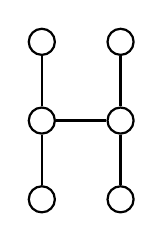
\begin{tikzpicture}[scale=1,
  thick,main node/.style={circle,draw,font=\sffamily\bfseries,minimum size=3mm}]

  \node[main node] (1) at (0,0) {};
  \node[main node] (2) at (0,1){};
  \node[main node] (3) at (0,2){};
  \node[main node] (4) at (1,0) {};
  \node[main node] (5) at (1,1) {};
  \node[main node] (6) at (1,2) {};

  \path[every node/.style={font=\sffamily\small}]
   (1) edge node[above]{}(2)
   (2) edge node[above]{}(3)
   (2) edge node[above]{}(5)
   (4) edge node[above]{}(5)
   (5) edge node[above]{}(6);
\end{tikzpicture}
\hskip10mm
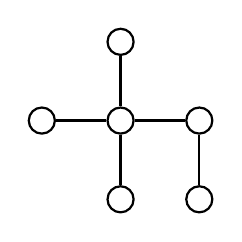
\begin{tikzpicture}[scale=1,
  thick,main node/.style={circle,draw,font=\sffamily\bfseries,minimum size=3mm}]

  \node[main node] (1) at (0,1) {};
  \node[main node] (2) at (1,0){};
  \node[main node] (3) at (1,1){};
  \node[main node] (4) at (1,2) {};
  \node[main node] (5) at (2,0) {};
  \node[main node] (6) at (2,1) {};

  \path[every node/.style={font=\sffamily\small}]
   (1) edge node[above]{}(3)
   (2) edge node[above]{}(3)
   (3) edge node[above]{}(6)
   (4) edge node[above]{}(3)
   (5) edge node[above]{}(6);
\end{tikzpicture}
\end{center}

\end{thm}
